% arara: pdflatex
% arara: bibtex
% arara: pdflatex
\documentclass{article}
\title{Mathematics for Machine Learning}
\author{Garrett Thomas\\
Department of Electrical Engineering and Computer Sciences\\
University of California, Berkeley}

% useful packages
\usepackage{amsfonts,amsmath,amssymb,amsthm,commath,enumerate,graphicx,hyperref}

% formatting
\setlength{\parskip}{0.5em}
\setlength{\parindent}{0em}
\usepackage[margin=1.25in]{geometry}
\hypersetup{
    colorlinks=true,
    linktoc=all,
    linkcolor=black,
    urlcolor=blue
}

% shorthand
\DeclareMathOperator*{\argmax}{arg\,max}
\DeclareMathOperator*{\argmin}{arg\,min}
\DeclareMathOperator*{\dom}{dom}
\DeclareMathOperator*{\range}{range}
\DeclareMathOperator*{\diag}{diag}
\DeclareMathOperator*{\tr}{tr}
\newcommand{\R}{\mathbb{R}}
\newcommand{\kwoo}[2]{\frac{\partial #1}{\partial #2}}
\newcommand{\kwoosq}[2]{\frac{\partial^2 #1}{\partial #2^2}}
\newcommand{\kwootwo}[3]{\frac{\partial^2 #1}{\partial #2 \partial #3}}
\newcommand{\mat}[1]{\begin{bmatrix}#1\end{bmatrix}}
\newcommand{\tran}{^\text{T}}
\newcommand{\inner}[2]{\langle #1, #2 \rangle}
\newcommand{\pr}[1]{\mathbb{P}(#1)}
\newcommand{\ev}[1]{\mathbb{E}[#1]}
\newcommand{\evwrt}[2]{\mathbb{E}_{#1}[#2]}
\newcommand{\var}[1]{\operatorname{Var}(#1)}
\newcommand{\cov}[2]{\operatorname{Cov}(#1, #2)}
\newcommand{\bigpr}[1]{\mathbb{P}\left(#1\right)}
\newcommand{\bigev}[1]{\mathbb{E}\left[#1\right]}
\newcommand{\bigvar}[1]{\operatorname{Var}\left(#1\right)}
\newcommand{\bigcov}[2]{\operatorname{Cov}\left(#1, #2\right)}
\newcommand{\iid}{\overset{iid}{\sim}}
\newcommand{\bX}{\mathbf{X}}
\newcommand{\term}[1]{\textbf{#1}}
\newcommand{\tab}{\hspace{0.5cm}}

\begin{document}
\maketitle

\section{About}
Machine learning uses tools from a variety of mathematical fields. This document is intended to summarize the mathematical background needed for an introductory class in machine learning, which at UC Berkeley is known as CS 189. We will cover topics in multivariable calculus/optimization, linear algebra, and probability. Our assumption is that the reader is already familiar with single-variable calculus and has encountered the basic concepts of multivariable calculus and linear algebra (at the level of UCB Math 53/54). We emphasize that this document is \textbf{not} a replacement for the prerequisite classes.

You are free to distribute this document as you wish. Please report any mistakes to \url{gwthomas@berkeley.edu}.

\newpage
\tableofcontents

\newpage
\section{Notation}
\begin{tabular}{|l|l|}
\hline
Notation & Meaning \\
\hline
$\R$ & the set of real numbers \\
$\R^n$ & the set (vector space) of $n$-tuples of real numbers, endowed with the usual inner product \\
$\R^{m \times n}$ & the set (vector space) of $m$-by-$n$ matrices \\
$\nabla f(x)$ & the gradient of the function $f$ evaluated at some point $x$ \\
$\nabla^2 f(x)$ & the Hessian of the function $f$ evaluated at some point $x$ \\
$A\tran$ & the transpose of the matrix $A$ \\
$\Omega$ & sample space \\
$\pr{A}$ & the probability of event $A$ \\
$\pr{A \mid B}$ & the probability of event $A$, given $B$ \\
$A^c$ & the complement of event $A$ \\
$\ev{X}$ & the expected value of random variable $X$ \\
$\var{X}$ & the variance of random variable $X$ \\
$\cov{X}{Y}$ & the covariance of random variables $X$ and $Y$ \\
$|S|$ & cardinality of set $S$ \\
\hline
\end{tabular}

\vspace{0.5cm}
Other notes:
\begin{itemize}
\item We will restrict ourselves to real values. In many places in this document, it is entirely possible (and in fact natural) to generalize to the complex case, but we will simply state the version that applies to the reals.

\item We assume that vectors are column vectors, i.e. that a vector in $\R^n$ can be interpreted as an $n$-by-$1$ matrix. As such, taking the transpose of a vector is well-defined (and produces a row vector, which is a $1$-by-$n$ matrix).

\item We do not provide proofs of most of the theorems given in this document. The proofs are not the point -- our primary goal is to review important definitions and concepts.
\end{itemize}

\newpage
\section{Calculus and optimization}
Much of machine learning is about minimizing a \term{cost function} (also called an \term{objective function} in the optimization community), which is a scalar function of several variables that typically measures how poorly our model fits the data we have. We will not give specific examples of cost functions here (go to class for these!) but we will assume here that our cost function has the form $f : \R^n \to \R$ and is sufficiently differentiable.

\subsection{Gradients}
The single most important concept from calculus in the context of machine learning is the \term{gradient}. Gradients are a generalization of the derivative to scalar functions of several variables. The gradient of $f(x_1, \dots, x_n)$, denoted $\nabla f$, is given by
\[\nabla f = \mat{\kwoo{f}{x_1} \\ \vdots \\ \kwoo{f}{x_n}}\]
Gradients have a very important property: $\nabla f$ points in the direction of \term{steepest ascent}:
\begin{center}
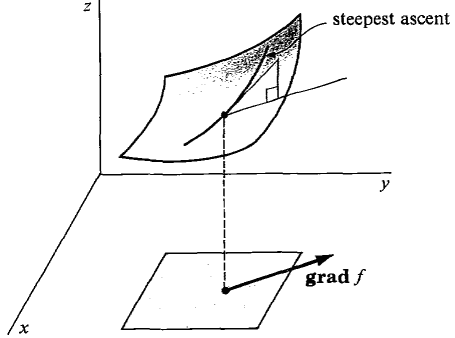
\includegraphics[width=0.9\linewidth]{gradient.png}
\end{center}
We will use this fact frequently when iteratively minimizing a function via \term{gradient descent}:
\[\theta_{k+1} = \theta_k - \eta_k \nabla f(\theta_k)\]
where $\eta_k > 0$ is called the \term{step size}.

\subsection{Hessians}
The \term{Hessian} is a matrix of second-order partial derivatives:
\[\nabla^2 f = \mat{
	\kwoosq{f}{x_1} & \hdots & \kwootwo{f}{x_1}{x_n} \\
	\vdots & \ddots & \vdots \\
	\kwootwo{f}{x_n}{x_1} & \hdots & \kwoosq{f}{x_n}
}\]
i.e. $(\nabla^2 f)_{ij} = \kwootwo{f}{x_i}{x_j}$. The Hessian is used in some optimization algorithms, such as Newton's method. It is expensive to calculate but can drastically reduce the number of iterations needed to converge to a local minimum by providing information about the curvature of $f$.

\subsection{Extrema}
Optimization is about finding \term{extrema}, which depending on the application could be minima or maxima. A point $x$ is said to be a \term{local minimum} of $f$ if $f(x) \leq f(y)$ for all $y$ in some neighborhood about $x$, and similarly a \term{local maximum} of $f$ if $f(x) \geq f(y)$ for all $y$ in some neighborhood about $x$. Furthermore, if $f(x) \leq f(y)$ for all $y$ in the entire domain of $f$, then $x$ is a \term{global minimum} of $f$ (similarly for global maximum).

Here is a useful criterion: if $f$ is differentiable, then for any extremum $x$, $\nabla f(x) = 0$. Note that the converse does not hold in general, that is, $\nabla f(x) = 0$ does not imply that $x$ is an extremum. It could be a \term{saddle point} of $f$.

\subsection{Convexity}
A function $f$ is said to be \term{convex} if
\[f(\lambda x + (1-\lambda)y) \leq \lambda f(x) + (1-\lambda)f(y)\]
for all $x, y \in \dom f$ and any $\lambda \in [0,1]$. Geometrically, this means that the line segment between two points on the graph of $f$ lies on or above the graph itself:
\begin{center}
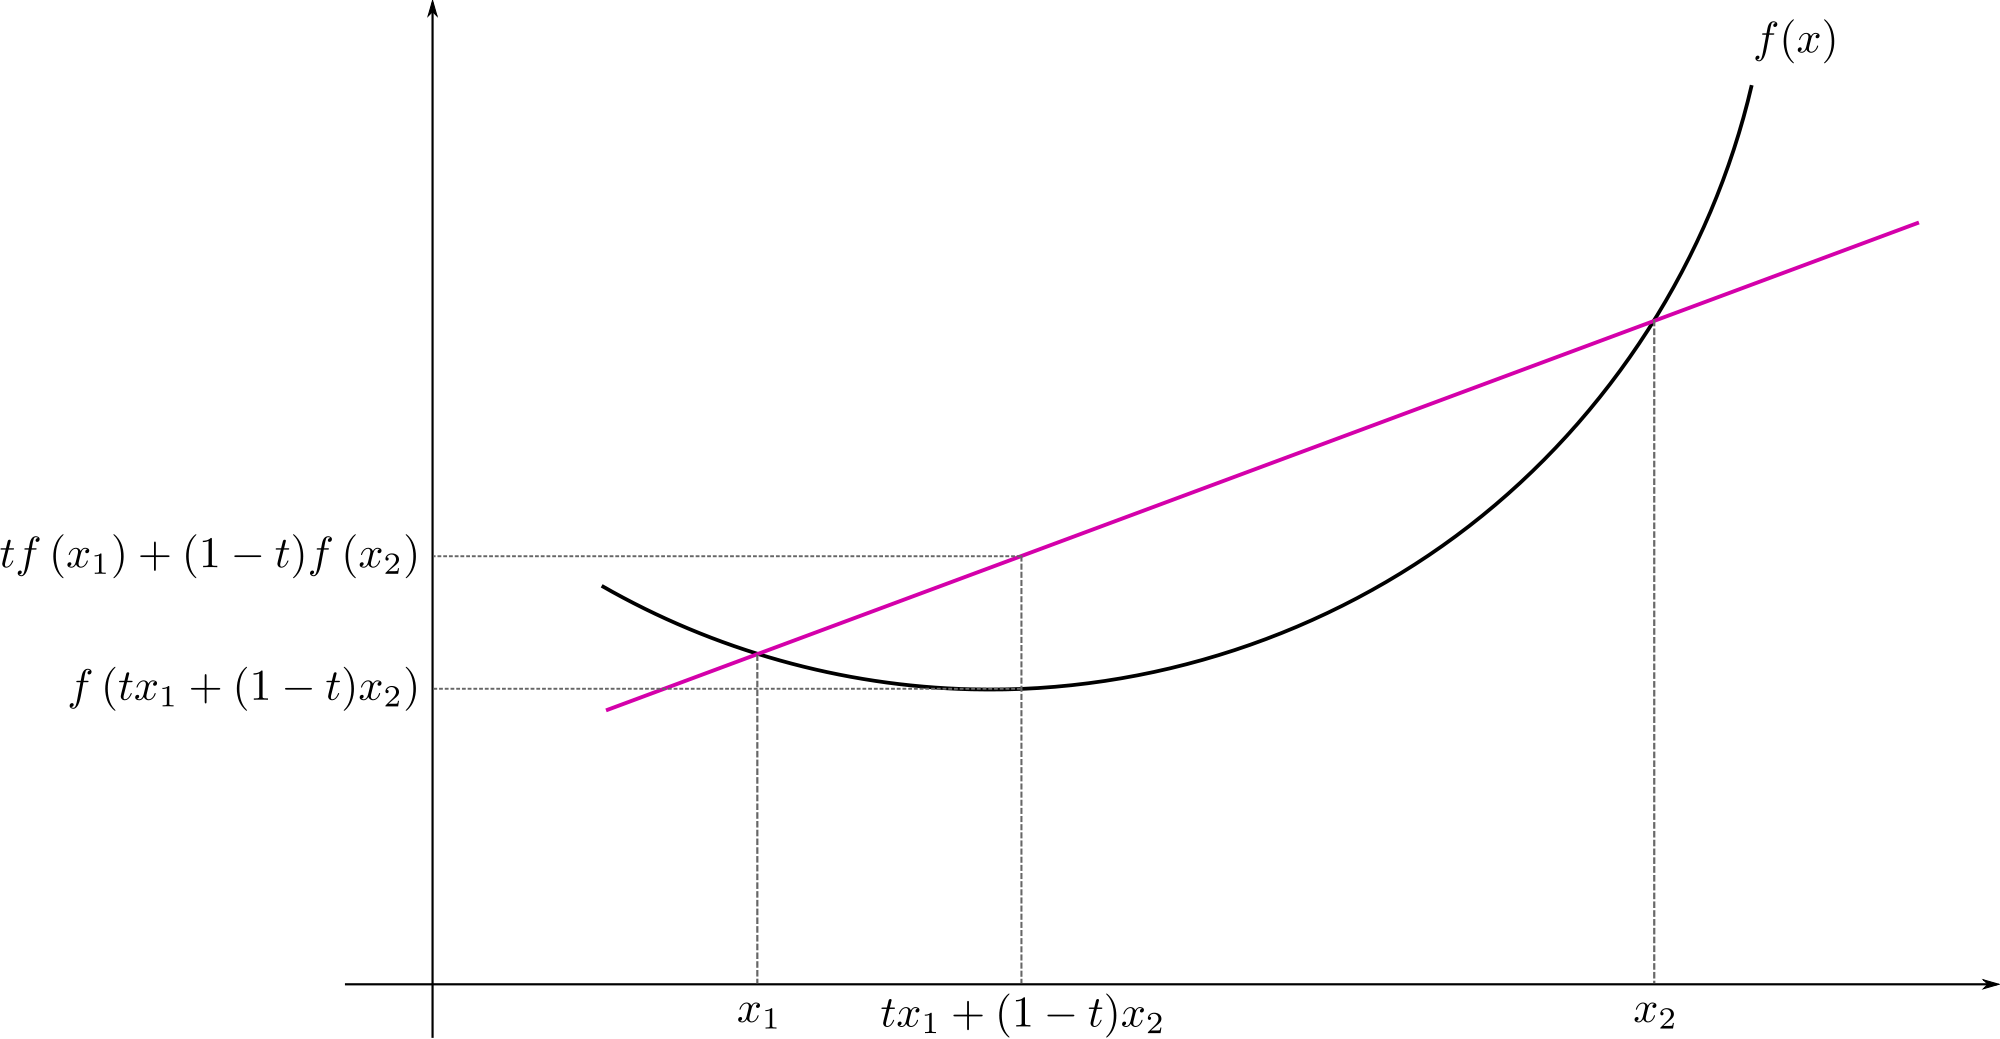
\includegraphics[width=0.9\linewidth]{convex}
\end{center}
We say that a function is \term{concave} if its negation is convex.

There are a number of ways to show that a function is convex:
\begin{enumerate}[(i)]
\item If $f$ is differentiable, then it is convex on an interval if and only if its derivative is non-decreasing on that interval.
\item If $f$ is continuously differentiable, then it is convex on an interval if and only if
\[f(x) \geq f(y) + f'(y)(x-y)\]
for all $x,y$ in the interval.
\item If $f$ is twice differentiable, then it is convex on some convex set if and only if the Hessian $\nabla^2 f$ is positive semi-definite on the interior of that set.
\item If $f$ is convex and $c \geq 0$, then $cf$ is convex.
\item If $f$ and $g$ are convex, then $f+g$ is convex.
\item If $f$ is convex, then $g(x) \equiv f(Ax + b)$ is convex.
\item If $f$ and $g$ are convex, then $h(x) \equiv \max\{f(x),g(x)\}$ is convex.
\end{enumerate}

Convexity sounds at first like a very mysterious property, but it has some wonderful implications. A particularly nice consequence is that any local minimum of a convex function $f$ is a global minimum of $f$.

Unfortunately, many loss functions that we would like to minimize are non-convex. This means whatever local minima our optimization algorithm finds may not be globally optimal.

\newpage
\section{Linear Algebra}
\subsection{Eigenthings}
For a square matrix $A \in \R^{n \times n}$, there may be vectors which, when $A$ is applied to them, are simply scaled by some constant. Mathematically we say that a nonzero vector $x \in \R^n$ is an \term{eigenvector} of $A$ corresponding to \term{eigenvalue} $\lambda \in \R$ if $Ax = \lambda x$. (We exclude the zero vector from this definition because $A(0) = \lambda \cdot 0$ for every $\lambda \in \R$.)

Suppose $\lambda_1, \dots, \lambda_k$ are the eigenvalues of $A$. The \term{trace} and \term{determinant} of $A$ are the sum and product (respectively) of all $A$'s eigenvalues:
\[\tr(A) = \sum_{i=1}^k \lambda_i, ~ \det(A) = \prod_{i=1}^k \lambda_i\]

\subsection{Transposition}
If $A \in \R^{m \times n}$, its \term{transpose} $A\tran \in \R^{n \times m}$ is given by $(A\tran)_{ij} = A_{ji}$ for each $(i, j)$. In other words, the columns of $A$ become the rows of $A\tran$, and the rows of $A$ become the columns of $A\tran$.

The transpose has several nice algebraic properties that can be easily verified from the definition:
\begin{enumerate}
\item $(A\tran)\tran = A$
\item $(A+B)\tran = A\tran + B\tran$
\item $(AB)\tran = B\tran A\tran$
\item $(\alpha A)\tran = \alpha A\tran$
\end{enumerate}

\subsection{Norms}
Norms generalize the notion of length from Euclidean space.

A \term{norm} on some real vector space $V$ is a function $\|\cdot\| : V \to \R$ that satisfies
\begin{enumerate}
\item $\|x\| \geq 0$, with $\|x\| = 0$ if and only if $x = 0$
\item $\|\alpha x\| = |\alpha|\|x\|$
\item $\|x+y\| \leq \|x\| + \|y\|$ (the so-called \term{triangle inequality})
\end{enumerate}
for all $x,y \in V$ and all $\alpha \in \R$.

We will typically only be concerned with a few specific norms on $\R^n$:
\begin{align*}
\|x\|_1 &= \sum_{i=1}^n |x_i| \\
\|x\|_2 &= \sqrt{\sum_{i=1}^n x_i^2} \\
\|x\|_p &= \left(\sum_{i=1}^n |x_i|^p\right)^\frac{1}{p} \tab\tab (p \geq 1) \\
\|x\|_\infty &= \max_{1 \leq i \leq n} |x_i|
\end{align*}
Note that the 1- and 2-norms are special cases of the $p$-norm, and the $\infty$-norm is the limit of the $p$-norm as $p$ tends to infinity.

Here's a fun fact: for any given finite-dimensional vector space $V$, all norms on $V$ are equivalent in the sense that for two norms $\|\cdot\|_A, \|\cdot\|_B$, there exist constants $\alpha, \beta \in \R$ such that
\[\alpha\|x\|_A \leq \|x\|_B \leq \beta\|x\|_A\]
for all $x \in V$.

\subsection{Inner Products}
An \term{inner product} on some real vector space $V$ is a function $\inner{\cdot}{\cdot} : V \times V \to \R$ satisfying
\begin{enumerate}
\item $\inner{x}{x} \geq 0$, with $\inner{x}{x} = 0$ if and only if $x = 0$
\item $\inner{\alpha x + \beta y}{z} = \alpha\inner{x}{z} + \beta\inner{y}{z}$
\item $\inner{x}{y} = \inner{y}{x}$
\end{enumerate}
for all $x,y,z \in V$ and all $\alpha,\beta \in \R$. When a vector space is endowed with an inner product, it is called an \term{inner product space}.

Note that any inner product on $V$ induces a norm on $V$:
\[\|x\| = \sqrt{\inner{x}{x}}\]
One can verify that the norm axioms are satisfied under this definition and follow directly from the axioms for inner products. 

Two vectors $x$ and $y$ are said to be \term{orthogonal} if $\inner{x}{y} = 0$. Orthogonality generalizes the notion of perpendicularity from Euclidean space. If two orthogonal vectors $x$ and $y$ additionally have unit length (i.e. $\|x\| = \|y\| = 1$), then they are described as \term{orthonormal}.

The standard inner product of $x, y \in \R^n$ is denoted $x\tran y$ (or $x \cdot y$, hence the alternative name \term{dot product}) and is given by
\[x\tran y = \sum_{i=1}^n x_iy_i\]
This notation arises because this inner product is a special case of matrix multiplication where we regard the resulting $1 \times 1$ matrix as a scalar. The reader can also verify that the two-norm $\|\cdot\|_2$ on $\R^n$ is induced by this inner product.

\subsection{Pythagorean Theorem}
The well-known Pythagorean theorem generalizes naturally to arbitrary inner product spaces: if $\inner{x}{y} = 0$, then
\[\|x+y\|^2 = \|x\|^2 + \|y\|^2\]
\begin{proof}
Suppose $\inner{x}{y} = 0$. Then
\[\|x+y\|^2 = \inner{x+y}{x+y} = \inner{x}{x} + \inner{y}{x} + \inner{x}{y} + \inner{y}{y} = \|x\|^2 + \|y\|^2\]
as claimed.
\end{proof}

\subsection{The Cauchy-Schwarz Inequality}
This inequality is sometimes useful in proving bounds:
\[|\inner{x}{y}| \leq \|x\| \cdot \|y\|\]
for all $x, y \in V$. Equality holds exactly when $x$ and $y$ are scalar multiples of each other (or equivalently, when they are linearly dependent).

\subsection{Special Kinds of Matrices}
There are several ways matrices can be classified. Each categorization implies some potentially desirable properties, so it's always good to know what kind of matrix you're dealing with.

\subsubsection{Orthogonal Matrices}
A matrix $Q \in \R^{n \times n}$ is said to be \term{orthogonal} if its columns are pairwise orthonormal. This definition implies that
\[Q\tran Q = QQ\tran = I\]
or equivalently, $Q\tran = Q^{-1}$. A nice thing about orthogonal matrices is that they preserve inner products:
\[(Qx)\tran(Qy) = x\tran Q\tran Qy = x\tran I y = x\tran y\]
A direct result of this fact is that orthogonal matrices also preserve 2-norms:
\[\|Qx\|_2 = \sqrt{(Qx)\tran(Qx)} = \sqrt{x\tran x} = \|x\|_2\]

\subsubsection{Symmetric Matrices}
A matrix $A \in \R^{n \times n}$ is said to be \term{symmetric} if it is equal to its own transpose ($A = A\tran$). A very important property of symmetric matrices is that they can be decomposed in the following manner:
\[A = Q\Lambda Q\tran\]
Here $Q$ is an orthogonal matrix, and $\Lambda = \diag(\lambda_1, \dots, \lambda_n)$, where $\lambda_1, \dots, \lambda_n$ are the eigenvalues of $A$. This is referred to as the \term{eigendecomposition} or \term{spectral decomposition} of $A$.

\subsubsection{Positive (Semi-)Definite Matrices}
A symmetric matrix $A$ is \term{positive definite} if for all nonzero $x \in \R^n$, $x\tran Ax > 0$. Sometimes people write $A > 0$ to indicate that $A$ is positive definite. Positive definite matrices have all positive eigenvalues.

A symmetric matrix $A$ is \term{positive semi-definite} if for all $x \in \R^n$, $x\tran Ax \geq 0$. Sometimes people write $A \geq 0$ to indicate that $A$ is positive semi-definite. Positive semi-definite matrices have all nonnegative eigenvalues.

Positive definite and positive semi-definite matrices will come up very frequently! Note that since these matrices are also symmetric, the properties of symmetric matrices apply here as well.

As an example of how these matrices arise, the matrix $A\tran A$ is positive semi-definite for any $A \in \R^{m \times n}$, since
\[x\tran (A\tran A)x = (Ax)\tran(Ax) = \|Ax\|_2^2 \geq 0\]
for any $x \in \R^n$.

\subsection{Singular Value Decomposition}
Singular value decomposition (SVD) is a widely applicable tool in linear algebra. Its strength stems partially from the fact that \textit{every matrix} $A \in \R^{m \times n}$ has an SVD (even non-square matrices)! The decomposition goes as follows:
\[A = U\Sigma V\tran\]
where $U \in \R^{m \times m}$ and $V \in \R^{n \times n}$ are orthogonal matrices and $\Sigma \in \R^{m \times n}$ is a diagonal matrix\footnote{Some would protest that a diagonal matrix must be square. We simply mean that all the off-diagonal entries are zero.} with the \term{singular values} of $A$ (denoted $\sigma_i$) on its diagonal. By convention, the singular values are given in non-increasing order, i.e.
\[\sigma_1 \geq \sigma_2 \geq \dots \geq \sigma_{\min(m,n)} \geq 0\]
Only the first $r$ singular values are nonzero, where $r$ is the rank of $A$.

The singular values of $A$ are the square roots of the eigenvalues of $A\tran A$ (or equivalently, of $AA\tran$).

The columns of $U$ are called the \term{left-singular vectors} of $A$, and they are eigenvectors of $AA\tran$. (Try showing this!) The columns of $V$ are called the \term{right-singular vectors} of $A$, and they are eigenvectors of $A\tran A$.

There is another useful way to write the SVD:
\[A = \sum_{i=1}^r \sigma_i u_i v_i\tran\]

\newpage
\section{Probability}
Probability theory provides powerful tools for modeling and dealing with uncertainty. In machine learning, we will use it extensively, particularly to construct and analyze classifiers.

\subsection{Basics}
Suppose we have some sort of randomized experiment (e.g. a coin toss, die roll) that has a fixed set of possible outcomes.  We call this set the \term{sample space} and denote it $\Omega$. Any subset $A \subseteq \Omega$ is called an \term{event}.
A \term{probability distribution} over $\Omega$ specifies how likely each event is to occur. We write $\pr{A}$ for the probability of event $A$.

Here are the basic axioms of probability:
\begin{enumerate}
\item For any event $A \subseteq \Omega$, $\pr{A} \geq 0$
\item $\pr{\Omega} = 1$
\item If $A_1, \dots, A_n$ are \term{mutually exclusive}, i.e. $A_i \cap A_j = \varnothing$ for $i \neq j$, then
\[\pr{A_1 \cup \cdots \cup A_n} = \pr{A_1} + \cdots + \pr{A_n}\]
\end{enumerate}
From these axioms, a number of useful rules can be derived (see \cite{pitman}):
\begin{enumerate}
\item $\pr{\varnothing} = 0$
\item If $A \subseteq B$, then $\pr{A} \leq \pr{B}$
\item $\pr{A} + \pr{A^c} = 1$
\item $\pr{A \cup B} = \pr{A} + \pr{B} - \pr{A \cap B}$
\end{enumerate}

\subsubsection{Conditional Probability}
The \term{conditional probability} of event $A$ given that event $B$ has occurred is written $\pr{A \mid B}$ and defined as
\[\pr{A \mid B} = \frac{\pr{A \cap B}}{\pr{B}}\]
assuming $\pr{B} > 0$.

\subsubsection{Chain Rule}
Another very useful tool, the \term{chain rule}, follows immediately from this definition:
\[\pr{A \cap B} = \pr{A \mid B}\pr{B} = \pr{B \mid A}\pr{A}\]

\subsubsection{Bayes' Rule}
Taking the equality from above one step further, we arrive at the simple but crucial \term{Bayes' rule}:
\[\pr{A \mid B} = \frac{\pr{B \mid A}\pr{A}}{\pr{B}}\]
It is sometimes beneficial to omit the normalizing constant and write
\[\pr{A \mid B} \propto \pr{A}\pr{B \mid A}\]
Under this formulation, $\pr{A}$ is often referred to as the \term{prior} and $\pr{B \mid A}$ as the \term{likelihood}.

In the context of machine learning, we can use Bayes' rule to update our ``beliefs'' (e.g. values of our model parameters) given some data that we've observed.

\subsection{Random Variables}
A \term{random variable} (r.v.) is some uncertain quantity with an associated probability distribution over the values it can assume. We write $X \sim p(\cdot)$ to indicate that the random variable $X$ is distributed according to some probability mass/density function $p$ (more on these functions below).

Formally, a random variable is a function from the sample space $\Omega$ to some other set of values, which we denote $X(\Omega) = \{X(\omega) \mid \omega \in \Omega\}$. To give a concrete example (taken from Pitman), suppose $X$ is the number of heads in two tosses of a fair coin. The sample space is
\[\Omega = \{hh, tt, ht, th\}\]
and $X$ is determined completely by the outcome $\omega$, i.e. $X = X(\omega)$. Moreover, we see the fundamental way that a random variable relates back to its underlying sample space:
\[\pr{X = x} = \pr{\{\omega \in \Omega \mid X(\omega) = x\}}\]
Typically we work only with random variables and don't concern ourselves with the original sample space $\Omega$, but it's worth knowing that it really is there behind the scenes.

A word on notation: we write $p(X)$ to denote the entire probability distribution of $X$ and $p(x)$ for the evaluation of the function $p$ at a particular value $x \in X(\Omega)$. Hopefully this (reasonably standard) abuse of notation is not too distracting. If $p$ is parameterized by some parameters $\theta$, we write $p(X; \theta)$ or $p(x; \theta)$, unless we are in a Bayesian setting where the parameters are considered a random variable, in which case we condition on the parameters.

\subsubsection{Discrete Random Variables}
Discrete r.v.'s are usually specified by a nonnegative \term{probability mass function} (p.m.f.) $p$ which satisfies
\[\sum_{x \in X(\Omega)} p(x) = 1\]
For a discrete $X$, the probability of a particular value is given exactly by its p.m.f.:
\[\pr{X = x} = p(x)\]

\subsubsection{Continuous Random Variables}
Continuous r.v.'s are usually specified by a nonnegative \term{probability density function} (p.d.f.) $p$ which satisfies
\[\int_{X(\Omega)} p(x) \dif{x} = 1\]
For a continuous $X$, the probability of a particular value is zero ($\forall x \in X(\Omega)$, $\pr{X = x} = 0$), so to get a positive probability we must integrate the p.d.f. over some range of values:
\[\pr{a \leq X \leq b} = \int_a^b p(x)\dif{x}\]

\subsubsection{The Cumulative Distribution Function}
The \term{cumulative distribution function} (c.d.f.) gives the probability that a random variable is at most a certain value:
\[F_X(x) = \pr{X \leq x}\]
The c.d.f. can be used to give the probability that a variable lies within a certain range:
\[\pr{a < X \leq b} = F_X(b) - F_X(a)\]

\subsection{Joint Distributions}
Often we have several random variables and we would like to get a distribution over some combination of them. A \term{joint distribution} is exactly this. For some r.v.'s $X_1, \dots, X_n$, the joint distribution is written $p(X_1, \dots, X_n)$ and gives probabilities over entire assignments to all the $X_i$ simultaneously.

We say that two variables $X$ and $Y$ are \term{independent} if their joint distribution factors into their respective distributions, i.e.
\[p(X, Y) = p(X)p(Y)\]
It is often convenient (though perhaps questionable) to assume that a bunch of random variables are \term{independent and identically distributed} (i.i.d.) so that their joint distribution can be factored entirely:
\[p(X_1, \dots, X_n) = \prod_{i=1}^n p(X_i)\]
where $X_1, \dots, X_n$ all share the same p.m.f./p.d.f.

\subsubsection{Marginal Distributions}
If we have a joint distribution over some set of random variables, it is possible to obtain a distribution for a subset of them by ``summing out'' (or ``integrating out'' in the continuous case) the variables we don't care about:
\[p(X) = \sum_{y \in Y(\Omega_Y)} p(X, y)\]

\subsection{Great Expectations}
If we have some random variable $X$, we might be interested in knowing what is the ``average'' value of $X$. This concept is captured by the \term{expected value} (or \term{mean}) $\ev{X}$, which is defined as
\[\ev{X} = \sum_{x \in X(\Omega)} x p(x)\]
for discrete $X$ and as
\[\ev{X} = \int_{X(\Omega)} xp(x)\dif{x}\]
for continuous $X$.

In words, we are taking a weighted sum of the values that $X$ can take on, where the weights are the probabilities of those respective values. The expected value has a physical interpretation as the ``center of mass'' of the distribution.

\subsubsection{Properties of Expected Value}
A very useful property of expectation is that of linearity:
\[\bigev{\sum_{i=1}^n \alpha_i X_i + \beta} = \sum_{i=1}^n \alpha_i \ev{X_i} + \beta\]
Note that this holds even if the $X_i$ are not independent!

But if they are independent, the product rule also holds:
\[\bigev{\prod_{i=1}^n X_i} = \prod_{i=1}^n \ev{X_i}\]

\subsection{Variance}
Expectation provides a measure of the ``center'' of a distribution, but frequently we are also interested in what the ``spread'' is about that center. We define the variance $\var{X}$ of a random variable $X$ by
\[\var{X} = \bigev{\left(X - \ev{X}\right)^2}\]
In words, this is the average squared deviation of the values of $X$ from the mean of $X$. Using a little algebra and the linearity of expectation, it is straightforward to show that
\[\var{X} = \ev{X^2} - \ev{X}^2\]

\subsubsection{Properties of Variance}
Variance is not linear (because of the squaring in the definition), but one can show the following:
\[\var{\alpha X + \beta} = \alpha^2 \var{X}\]
Basically, multiplicative constants become squared when they are pulled out, and additive constants disappear (since the variance contributed by a constant is zero).

Furthermore, if $X_1, \dots, X_n$ are uncorrelated\footnote{We haven't defined this yet; see the Correlation section below}, then
\[\var{X_1 + \dots + X_n} = \var{X_1} + \dots + \var{X_n}\]

\subsubsection{Standard Deviation}
Variance is a useful notion, but our definition suffers from that fact the units of variance are not the same as the units of the random variable (again because of the squaring). To overcome this problem we can use \term{standard deviation}, which is defined as $\sqrt{\var{X}}$. The standard deviation has the same units as $X$.

\subsection{Covariance}
Covariance is a measure of the linear relationship between two random variables. We denote the covariance between $X$ and $Y$ as $\cov{X}{Y}$, and it is defined to be
\[\cov{X}{Y} = \ev{(X-\ev{X})(Y-\ev{Y})}\]
Note that the expectation must be taken over the joint distribution of $X$ and $Y$.

Again, the linearity of expectation allows us to rewrite this as
\[\cov{X}{Y} = \ev{XY} - \ev{X}\ev{Y}\]
Comparing these formulas to the ones for variance, it is not hard to see that $\var{X} = \cov{X}{X}$.

\subsubsection{Correlation}
Normalizing the covariance gives the \term{correlation}:
\[\rho(X, Y) = \frac{\cov{X}{Y}}{\sqrt{\var{X}\var{Y}}}\]
Correlation also measures the linear relationship between two variables, but unlike covariance always lies between $-1$ and $1$.

Two variables are said to be \term{uncorrelated} if $\cov{X}{Y} = 0$ because $\cov{X}{Y} = 0$ implies that $\rho(X, Y) = 0$. If two variables are independent, then they are uncorrelated, but the converse does not hold in general.

\subsection{Random Vectors}
So far we have been talking about \term{univariate distributions}, that is, distributions of single variables. But we can also talk about \term{multivariate distributions} which give distributions of \term{random vectors}:
\[\bX = \mat{X_1 \\ \vdots \\ X_n}\]
The metrics we have discussed for single variables have natural generalizations to the multivariate case.

Expectation of a random vector is simply the expectation applied to each component:
\[\ev{\bX} = \mat{\ev{X_1} \\ \vdots \\ \ev{X_n}}\]

The variance is generalized by the \term{covariance matrix}:
\[\Sigma = \ev{(\bX - \ev{\bX})(\bX - \ev{\bX})\tran} = \mat{
\var{X_1} & \cov{X_1}{X_2} & \hdots & \cov{X_1}{X_n} \\
\cov{X_2}{X_1} & \var{X_2} & \hdots & \cov{X_2}{X_n} \\
\vdots & \vdots & \ddots & \vdots \\
\cov{X_n}{X_1} & \cov{X_n}{X_2} & \hdots & \var{X_n}
}\]
We see $\Sigma_{ij} = \cov{X_i}{X_j}$. Since covariance is symmetric in its arguments, the covariance matrix is also symmetric. It's also positive semi-definite: for any $v$,
\[v\tran\Sigma v = v\tran\ev{(\bX - \ev{\bX})(\bX - \ev{\bX})\tran}v = \ev{v\tran(\bX - \ev{\bX})(\bX - \ev{\bX})\tran v} = \ev{\|(\bX - \ev{\bX})\tran v\|_2^2} \geq 0\]

The inverse of the covariance matrix, $\Sigma^{-1}$, is sometimes called the \term{precision matrix}.

\subsection{Estimation of Parameters}
Now we get into some basic topics from statistics. We make some assumptions about our problem by prescribing a \term{parametric} model (e.g. a distribution that describes how the data were generated), then we fit the parameters of the model to the data. How do we choose the values of the parameters?

\subsubsection{Maximum Likelihood Estimation}
A common way to fit parameters is \term{maximum likelihood estimation} (MLE). The basic principle of MLE is to choose values that ``explain'' the data best by maximizing the probability of the data we've seen, conditioned on the parameters. Suppose we have random variables $X_1, \dots, X_n$ and corresponding observations $x_1, \dots, x_n$. Then
\[\hat{\theta}_\textsc{mle} = \argmax_\theta \mathcal{L}(\theta)\]
where $\mathcal L$ is the \term{likelihood function}
\[\mathcal{L}(\theta) = p(x_1, \dots, x_n; \theta)\]
Often, we assume that $X_1, \dots, X_n$ are i.i.d. Then we can write
\[p(x_1, \dots, x_n; \theta) = \prod_{i=1}^n p(x_i; \theta)\]
At this point, it is usually convenient to take logs, giving rise to the \term{log-likelihood}
\[\log \mathcal{L}(\theta) = \sum_{i=1}^n \log p(x_i; \theta)\]
This is a valid operation because the probabilities/densities are assumed to be positive, and since log is a monotonically increasing function, it preserves ordering. In other words, any maximizer of $\log \mathcal L$ will also maximize $\mathcal L$.

For some distributions, it is possible to analytically solve for the maximum likelihood estimator. If $\log \mathcal L$ is differentiable, setting the derivatives to zero and trying to solve for $\theta$ is a good place to start.

\subsubsection{Maximum a Posteriori Estimation}
A more Bayesian way to fit parameters is through \term{maximum a posteriori estimation} (MAP). In this technique we assume that the parameters are a random variable, and we specify a prior distribution $p(\theta)$. Then we can employ Bayes' rule to compute the posterior distribution of the parameters given the observed data:
\[p(\theta \mid x_1, \dots, x_n) \propto p(\theta)p(x_1, \dots, x_n \mid \theta)\]
Computing the normalizing constant is often intractable, because it involves integrating over the parameter space, which may be very high-dimensional. Fortunately, if we just want the MAP estimate, we don't care about the normalizing constant! It does not affect which values of $\theta$ maximize the posterior. So we have
\[\hat{\theta}_\textsc{map} = \argmax_\theta p(\theta)p(x_1, \dots, x_n \mid \theta)\]
A particularly nice case is when the prior is chosen carefully such that the posterior comes from the same family as the prior. In this case the prior is called a \term{conjugate prior}. For example, if the likelihood is binomial and the prior is beta, the posterior is also beta. There are many conjugate priors; the reader may find this \href{https://en.wikipedia.org/wiki/Conjugate_prior#Table_of_conjugate_distributions}{table of conjugate priors} useful.

\newpage
\bibliography{references}
\addcontentsline{toc}{section}{References}
\bibliographystyle{ieeetr}
\nocite{*}
%\begin{thebibliography}{9}
%\bibitem{boydvandenberghe}
%Something
%\end{thebibliography}

\end{document}